\documentclass[a4paper]{book}

\usepackage[utf8]{inputenc}
\usepackage[T1]{fontenc}
\usepackage{hyperref}
\usepackage{graphicx}
\usepackage{float}
\usepackage{amsmath}
\usepackage{amssymb}
\usepackage{color}
\usepackage{caption}
\usepackage{listings}
\usepackage{geometry}
\geometry{rmargin=3.6cm,lmargin=3.6cm}% for the title page

\author{Charles HAMESSE}
\title{Techniques of Artificial Intelligence \\~\\ ECOLE POLYTECHNIQUE DE BRUXELLES\\}
\date{\today}

\newcounter{nalg}[section]
\DeclareCaptionLabelFormat{algocaption}{Algorithm \thenalg} % defines a new caption label as Algorithm x.y

\lstnewenvironment{algorithm}[1][] %defines the algorithm listing environment
{   
    \refstepcounter{nalg} %increments algorithm number
    \captionsetup{labelformat=algocaption,labelsep=colon} %defines the caption setup for: it ises label format as the declared caption label above and makes label and caption text to be separated by a ':'
    \lstset{ %this is the stype
        frame=tb,
        numbers=left, 
        mathescape=true,
        numberstyle=\tiny,
        basicstyle=\scriptsize, 
        keywordstyle=\color{black}\bfseries\em,
        keywords={,input, output, return, datatype, function, in, if, else, foreach, while, begin, for, each, end, not, true, false, and, or} %add the keywords you want, or load a language as Rubens explains in his comment above.
        numbers=left,
        xleftmargin=.04\textwidth,
        #1 % this is to add specific settings to an usage of this environment (for instnce, the caption and referable label)
    }
}
{}
\begin{document}

\begin{titlepage}
	\centering
	\vspace{1cm}
	{\scshape\LARGE École Polytechnique de Bruxelles \par}
	\vspace{2cm}
	{\scshape\Large INFO-H-410\par}
	\vspace{.5cm}
	{\huge\bfseries Techniques of Artificial Intelligence\par}
	\vspace{2cm}
	{\Large Hugues \textsc{Bersini}\par}
	\vfill
	Summarized by\par
	Charles \textsc{Hamesse}

	\vfill

% Bottom of the page
	{\large \today\par}
\end{titlepage}
\tableofcontents
\tableofcontents

\chapter{Introduction}
First, let's review a brief history of the origins of AI, its objectives and challenges met throughout the years. It is common to distinguish the old AI from the new, expliciting the breakthrough that happened in response to some \textit{failures} of the first type of AI.

\section{Old-fashioned AI}
\paragraph{Intelligence} It is first considered as a set of mental inferences, allowing the ability to make deductions, planning, mental simulations, reasoning, logics, and so on. Also, we distinguish rational intelligence from \textit{fake} intelligences, such as emotional intelligence, animal intelligence, embodied intelligence, collective intelligence. 
In other words, intelligence is described about IQ, chess, math, logical solving. All the rest is just skills.

\paragraph{The inferential engine} At this time, we're able to determine a general canvas and state the requirements of such an AI problem. Those are the following:
\begin{enumerate}
    \item Find the operators that can be applied: their pre-conditions need to match the current state of the world
    \item Select one the control strategy: in depth or in width, with heuristics or not
    \item Avoid looping
    \item Be able to backtrack
    \item Do that iteratively until you find the final state
\end{enumerate}
The solution of a planning problem is the sequence of operators. If several solutions are elligible, it is often the one having the shortest sequence of operators that will be optimal.


\paragraph{The failures} Man is embodied in his environment. He is a sophisticated sensori-motor process much before any cogitive process takes on. His perception is intrinsically and materially parallel. The sensori-motor processes essentially depends on
their biological grounding: parallel and adaptable.
The outside world is complex and to be able to cope with, a man requires an interface of similar complexity. But this complexity can be achieved by learning and experience rather than being handcrafted. Complex processes emerge from iterating simple mechanisms

\section{Today's AI}
Man possess 2 cognitive systems
\begin{enumerate}
    \item Parallel, automatic, unconscious, reflex, adaptable and very efficient. Based on neuronal hardware, for playing tennis, piano, becoming an expert, etc.
    \item Sequential, rigid, conscious and very laborious. Based on neuronal software, for playing chess, for testing IQ
\end{enumerate}
Man goes from one to the other in the cases of breakdowns in his
automatisms. Machine intelligence and human intelligence can be of different nature. For the machines today, recognizing a face is much more difficult than playing chess. But doesn’t Kasparov in part play chess like indeed we recognize a face?\\
~\\
We can describe the following trends:\\
AI $\rightarrow$ ALife \\
Software $\rightarrow$ Hardware \\
Cognitive Science $\rightarrow$ Biology
\paragraph{Summary} The animal hidden in each of us might be unavoidable on the road to intelligence. Our intellectual skills are embodied in our automatisms. They depart from there. In other words, don’t ever try to fully understand what a chair is without having ever sat in it. Also, a turn back is needed towards our biological interface with the outside world.

%%%%%%%%%%%%%%%%%%%%%%%%%%%%%%%%%%%%%%%%%%%%%%%%%%%%%%%
\chapter{State space search}
%%%%%%%%%%%%%%%%%%%%%%%%%%%%%%%%%%%%%%%%%%%%%%%%%%%%%%%
Search problems are described in terms of: \\
– An initial state. (e.g., initial chessboard, current positions of objects in world, current location) \\
– A target state.(e.g., winning chess position, target location) \\
– Some possible actions, that get you from one state to another. (e.g. chess move, robot action, simple change in location). \\
\linebreak
Search techniques systematically consider all possible action sequences to find a path from the initial to target state. The set of all possible states reachable from the initial state defines the search space. We can represent the search space as a tree.

\section{Exhaustive search algorithms}
We may use simple systematic search techniques, which try every possibility in systematic way. Those are referred to as brute force or blind techniques and include breadth first and depth first search among others.\\
\linebreak
The algorithms for breadth first and depth first search a very easy to implement. Both algorithms keep track of the list of nodes found. List is sometimes referred to as an agenda, but implemented using stack for depth first and a queue for breadth first.
\begin{algorithm}[caption={Breadth-first search.}, label={alg1}]
queue = {initial-state}
found = false
while queue not empty and not found
    remove the first node N from queue
    if N is a goal state
        found = true
    find all the successor nodes of N, and put them on the end of the queue
\end{algorithm}

\begin{algorithm}[caption={Depth-first search.}, label={alg2}]
stack = {initial-state}
found = false
while stack not empty and not found
    remove the first node N from stack
    if N is a goal state
        found = true
    find all the successor nodes of N, and put them on the end of the stack.
\end{algorithm}

\paragraph{Choice between algorithms} When is one technique more appropriate than the other? \\
– Shortest path? BF \\
– Is memory a problem? DF \\
– Need to find the solution quickly? It depends on the structure of the search tree. To avoid long paths in DF search, define a depth limit. To find shortest path quickly, change DF search to iterative deepening.

\paragraph{Extensions to basic algorithm} What if there are loops (i.e., we are search a graph)? How do you avoid (virtually) driving round and round in circles? Algorithm needs to keep track of which nodes have already been explored, and avoids redoing these nodes.

\begin{algorithm}[caption={Variation of depth-first search.}, label={alg3}]
stack = {initial-state}
visited = $\emptyset$
found = false
while stack not empty and not found
    remove the first node N from stack
    if N $\notin$ visited
        visited = visited $\cup$ N
        if N is a goal state
            found = true
        find all the successor nodes of N, and put them on the end of the stack.
\end{algorithm}


\section{Heuristic search algorithms}
Depth first and breadth first search turn out to be too inefficient for really complex problems. Instead, we turn to “heuristic search” methods, which do not
search the whole search space, but focus on promising areas.\\
\linebreak 
To identify promising areas, we need an \textbf{evaluation function}. The evaluation function scores a node in the search tree on how close it is to the goal/target state.
\begin{algorithm}[caption={Hill climbing.}, label={alg4}]
current_state = initial_state
while current_state $\neq$ goal-state $\vee$ no change in current state
    get the successors of current_state
    evaluate the successors and assign them a score
    if one of the successors is better than current_state
        then set the new-current state to be the successor with the best score
\end{algorithm}
This algorithm avoids loop, but may halt without success in local maximum.

\begin{algorithm}[caption={Best first search.}, label={alg5}]
agenda = {initial_state}
found = false
while agenda $\neq \emptyset$ and not found
    remove the best node N from agenda
    if N is a goal state
        found = true
    find all successor nodes of N, assign them a score, and put them on the agenda organised as a priority queue.
\end{algorithm}
Best first search algorithm works almost the same way as depth/breadth search algorithms, but we use a priority queue where nodes with high scores are taken of the queue first. Hence still exhaustive search and performance depends on the quality of the evaluation function.

\begin{algorithm}[caption={A*.}, label={alg6}]
agenda = {initial_state}
found = false
while agenda $\neq \emptyset$ and not found
    remove best node N from agenda
    if N is a goal state
        found = true
    for s in all successor nodes of n
        s.score  = cost(initial_state, s) + cost(s, goal_state)
    put all successor nodes on the agenda organised as a priority queue
\end{algorithm}
This algorithm is basically an extension of the best-first search, taking the total path length into account. The score is based on the predicted total path “cost”, that is, a sum of the cost/distance from initial to current node, and the predicted cost/distance to target node.\\
\linebreak
In BF search (if the cost of traversing a link is the same), the solution with the lowest cost will be found first, but it may take time. In DF search, a solution can be found quickly, yet it may not be a very good one. The A* algorithm finds a cheap solution quickly.

\paragraph{Summary} General search methods can be used to solve
complex problems, which are formulated in terms of initial and target state, and the primitive actions that take you from one state to next. Also, one may need to use heuristic search for complex problems, as search space can be too large.


\chapter{Concept learning}
This section describes the functioning of algorithms able to learn from examples, determine version spaces and implement the candidate elimination algorithm.
\section{The inductive learning hypothesis} Any hypothesis found to approximate the target function well over a sufficiently large set of training examples will also approximate the target function well over other unobserved examples.

\paragraph{An example problem} For the \textit{EnjoySport} problem, the canvas is the following (refer to the slides for the full problem description).\\
\textbf{Given:}\\
- Instances $X$ (e.g. possible days described by attributes Sky, AirTemp, Humidity, etc),\\
- Target function $c$: EnjoySport : $X \rightarrow {0, 1}$,\\
- Hypotheses $H$: conjunctions of literals (e.g. $\langle$?, Cold, High, ?, ?, ? $\rangle$),\\
- Training examples $D$: positive and negative examples of the target function $\langle x_1, c(x_1) \rangle, ..., \langle x_m, c(x_m) \rangle$.\\
\textbf{Determine:}\\
A hypothesis $h$ in H such that $h(x) = c(x)$ ~ $\forall x \in D$.


\begin{algorithm}[caption={Find-S.}, label={alg7}]
$h$ = most specific hypothesis in $H$
for each positive training instance $x$
    for each attribute constraint $a_i$ in $h$
        if $a_i$ satisfied by $x$
            do nothing
        else 
            replace $a_i$ by the next more  general constraint satisfied by $x$
return $h$
\end{algorithm}
This algorithm seeks the most restrictive (i.e most \textit{specific}) hypothesis that fits all the positive examples (negatives are ignored). This algorithm shows a few drawbacks:\\
- Can't tell whether it has learned concept\\
- Can't tell when training data inconsistent\\
- Picks a maximally specific $h$ (why?)\\
- Depending on $H$, there might be several!

\section{Version spaces} A hypothesis $h$ is consistent with a set of
training examples $D$ of target concept $c$ if and only if $h(x) = c(x)$ for each training example $\langle x, c(x) \rangle$ in $D$.
\begin{equation*}
    Consistent(h, D) \equiv (\forall \langle x, c(x) \rangle \in D) ~ h(x) = c(x) 
\end{equation*}
The version space, $VS_{H,D}$, with respect to hypothesis space $H$ and training examples $D$, is the subset of hypotheses from $H$ consistent with all training examples in $D$.
\begin{equation*}
    VS_{H, D} \equiv  \{ h \in H ~|~ Consistent(h, D) \}
\end{equation*}


\begin{algorithm}[caption={List-then-eliminate.}, label={alg8}]
$VS \leftarrow$  list containing every hypothesis in $H$
for each training example $\langle h(x), c(x) \rangle$
    remove from $VS$ any hypothesis $h$ for which $h(x) \neq c(x)$
return $VS$
\end{algorithm}

\paragraph{Representing version spaces} The general boundary, $G$, of version space $VS_{H, D}$ is the set of its maximally \textbf{general} members. The specific boundary, $S$, of $VS_{H, D}$ is the set of its maximally \textbf{specific} members. Every member of the version space lies between these boundaries:
\begin{equation*}
    VS_{H, D} = \{ h \in H ~|~ g \geq h \geq s,~ \forall s \in S,~ g \in G \}
\end{equation*}
where $x \geq y$ means $x$ is more general or equal to $y$.


\begin{algorithm}[caption={Candidate elimination.}, label={alg9}]
$G \leftarrow$ maximally general hypotheses in $H$
$S \leftarrow$ maximally specific hypotheses in $H$
for each training example $d$
    if $d$ is a positive example
        remove from $G$ any hypothesis inconsistent with $d$
        for each hypothesis $s \in S$ inconsistent with $d$
            $S \leftarrow S \setminus s$
            $S \leftarrow S \cup \{ all minimal generalizations h of s | Consistent(h, d) \wedge  some member of G is more general than h \}$
            $S \leftarrow S \setminus \{ h ~|~ h > s ~ \forall h \in H,~ s \in S \}$
    if $d$ is a negative example 
        remove from S any hypothesis inconsistent with d
        for each hypothesis g in G that is not consistent with d
            $G \leftarrow G \setminus g$
            $G \leftarrow G \cup \{all minimal specializations h of g | Consistent(h, d) \wedge some member of S is more specific than h \}$
            $G \leftarrow G \setminus \{ h ~|~ h < g ~ \forall h \in H,~ g \in G \}$

\end{algorithm}
To-do: notes on this algorithm

\section{Bias}
So far, we have three types of learners with different biases:
\begin{enumerate}
    \item Rote learner: store examples, classify $x$ if and only if it matches previously observed example.
    \item Version space candidate elimination algorithm
    \item Find-S algorithm
\end{enumerate}
\paragraph{An unbiased learner} The idea is to choose and $H$ that expresses every teachable concept (i.e. $H$ is the power set of $X$, $2^X$).

\paragraph{Inductive bias} Let's consider concept learning algorithm $L$, a set of instances $X$, a target concept $c$, a set of training examples $D_c = \{ \langle x, c(x) \rangle \}$. Let $L(x_i, D_c)$ denote the classification assigned to the instance $x_i$ by $L$ after training on data $D_c$.\\
\linebreak The inductive bias of $L$ is any minimal set of assertions $B$ such that for any target
concept $c$ and corresponding training
examples $D_c$:
\begin{equation*}
(\forall x_i \in X) [ ( B \wedge D_c \wedge x_i) \vdash L(x_i, D_c)]
\end{equation*}
where $A \vdash B$ means $A$ logically entails $B$

\begin{figure}[h]
    \centering
    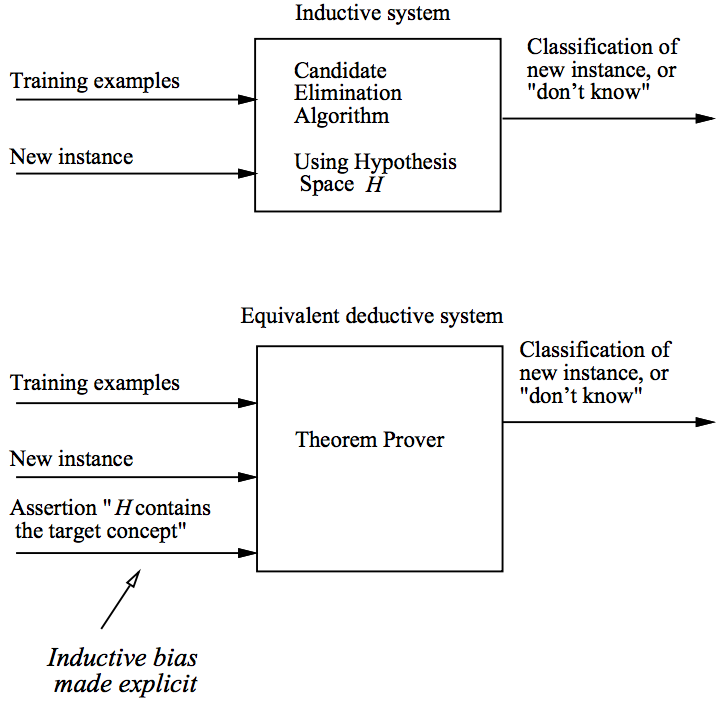
\includegraphics[width=0.7\linewidth]{img/inductivebias}
\end{figure}

\paragraph{Summary Points}
\begin{enumerate}
    \item Concept learning as search through $H$
    \item General-to-specific ordering over $H$
    \item Version space candidate elimination algorithm
    \item $S$ and $G$ boundaries characterize learner's uncertainty
    \item Learner can generate useful queries
    \item Inductive leaps possible only if learner is biased
    \item Inductive learners can be modelled by equivalent deductive systems
\end{enumerate}
\chapter{Decisions trees}
Decision trees are another formalism we can use to solve problems using learning algorithms. We may consider using decision trees when:
\begin{enumerate}
    \item Instances are describable by (attribute,value) pairs
    \item Target function is discrete valued
    \item Disjunctive hypothesis may be required
    \item Training date is possibly noisy
\end{enumerate}
For example, such trees are used for equipment or medical diagnosis, credit risk analysis, modeling calendar scheduling preferences, etc.

\section{Decision tree representation}
The representation of decision trees include the following features:
\begin{enumerate}
    \item Each internal node tests an attribute
    \item Each branch corresponds to an attribute value
    \item Each leaf node assigns a classification
\end{enumerate}

\begin{algorithm}[caption={Top-down induction of decision trees  (main loop).}, label={alg10}]
$A \leftarrow$ the "best" decision attribute for next node
assign A as decision attribute for node
for each value of A 
    create new descendant of node
sort training examples to leaf nodes
if training examples perfectly classified
    stop
else
    iterate over new leaf nodes
\end{algorithm}

\section{Entropy, information gain}
\paragraph{Entropy} Let's consider a set of training examples $S$. We can denote $p_{\oplus}$, the proportion of positive examples in $S$ and $p_{\ominus}$, the proportion of negative samples. The entropy is written:
\begin{equation*}
    Entropy(S) \equiv -p_{\oplus} log_2 p_{\oplus} - p_{\ominus} log_2 p_{\ominus}    
\end{equation*}
It represents the expected number of bits needed to encode a class ($p_{\oplus}$ or $p_{\ominus}$) of randomly drawn members of $S$ (under the optimal, shortest-length code), be cause an optimal length code assigns $-log_2 p$ bits to message having probability $p$. \\
\linebreak
\textit{Note:} a more general way to write entropy is:
\begin{equation*}
    Entropy(S) \equiv - \sum_{x \in X} p(x) \log_{2} p(x)     
\end{equation*}

\paragraph{The information gain} $Gain(S, A)$ is the expected reduction in entropy due to sorting the set $S$ on the attribute $A$. It is computed with:
\begin{equation*}
    Gain(S, A) \equiv Entropy(S) - \sum_{v \in  Values(A)} \frac{|S_v|}{|S|} Entropy(S_v)    
\end{equation*}

\section{ID3 learning algorithm}
\begin{algorithm}[caption={ID3.}, label={alg10}]
ID3(Examples $S$, Target_Attribute $t$, Attributes $A$)
    root $\leftarrow$ new root node for the tree
    if $s_i$ positive $\forall s_i \in S$
        return single-node tree root, labeled +.
    else if $s_i$ negative $\forall s_i \in S$
        return single-node tree root, labeled -.
    else if $|A| = 0$    
        return the single node tree root, labeled with the most common value of $t$ in $S$
    else
        $a \leftarrow \text{arg~max}~Gain(S, a_i) ~ \forall a_i \in A$
        for each value $v_i$ of $a$
            $b_i \leftarrow $ new tree branch below root, labeled $v_i$
            $Sv_i \leftarrow \{ s \in S ~|~ value(s, a) = v_i \}$ 
            if $Sv_i = \emptyset$
                add new leaf node below $b_i$ labeled with the most common target value in $S$
            else
                add new subtree below $b_i$ ID3 ($Sv_i$, $a$, $A \setminus \{a\}$)
    return root

\end{algorithm}
ID3 (Iterative Dichotomiser 3) is an algorithm used to generate a decision tree from a dataset. 
\paragraph{Properties of ID3}
\begin{enumerate}
    \item The hypothesis search space is complete. That is, the target function is surely there.
    \item Its choices are statistically based, i.e the algorithm is robust to noisy data.
    \item It does not guarantee an optimal solution; it can get stuck in local optima. It uses a greedy on each splitting iteration. We could use backtracking to find an optimal decision tree. 
    \item It can overfit to the training data. To avoid overfitting, smaller decision trees with high information gain attributes near the root should be preferred over larger ones (note that this algorithm usually produces small trees).
    \item It is harder to use on continuous data. Searching for the best value to split by can be time consuming.
\end{enumerate}
\paragraph{Inductive bias in ID3} Bias is a preference for some hypotheses, rather than a restriction of hypothesis space $2^X$ (the power set of instances $X$).
\paragraph{Attributes with many values} If an attribute has many possible values, $Gain(S, A)$ might select it over others that might be more appropriate (e.g. attribute, pairs such as "date = June 3, 1996"). One approach is to use the $GainRatio(S, A)$ instead: 
\begin{equation*}
    GainRatio(S, A) \equiv \frac{Gain(S, A)}{SplitInformation(S, A)}
\end{equation*}
together with
\begin{equation*}
    SplitInformation(S, A) \equiv -\sum_{i =1}^{c} \frac{|S_i|}{|S|} log_2 \frac{|S_i|}{|S|}    
\end{equation*}
where $S_i = \{ s \in S ~|~ value(s, A) = v_i \} $

\paragraph{Attributes with Costs} In some cases, attributes may come together with a cost. For example:\\
- Medical diagnosis, $BloodTest$ has cost EUR150\\
- Robotics, $Width\_from\_1ft$ has cost 23sec.\\
\linebreak
So how could we learn a consistent tree with low expected cost? There are two approaches based on the same idea: to replace gain by a function of itself and the cost.
\begin{enumerate}
    \item Tan and Schlimmer (1990)
    \begin{equation*}
        Gain(S,A) \rightarrow \frac{Gain^2 (S,A)}{Cost(A)}
    \end{equation*}
    \item Nunez (1988)
    \begin{equation*}
        Gain(S,A) \rightarrow \frac{2^{Gain (S,A)} - 1}{(Cost(A) + 1)^w}
    \end{equation*}
    where $w \in [0, 1]$ determines importance of cost.
\end{enumerate}

\paragraph{Unknown Attribute Values} What if some examples missing values of A? We may consider using training examples anyway, sort through the three considering the following aspects:
\begin{enumerate}
    \item If node $n$ tests $A$, assign most common value of $A$ among other examples sorted to node $n$
    \item Assign most common value of $A$ among other examples with same target value
    \item Assign probability $p_i$ to each possible value $v_i$ of $A$, and assign fraction $p_i$ of example to each descendant in tree.
    \item Classify new examples in the same fashion
\end{enumerate}


\section{Overfitting}

\paragraph{Occam's razor} It is a problem-solving principle: \textit{"prefer the shortest hypothesis that fits the data"}. Note that there exist several formulations. Then comes the question, why prefer short hypotheses? Well, a short hypothesis that fits data is unlikely a coincidence, whereas a long hypothesis that fits data might be coincidence with higher probability. However,  there are many ways to define small sets of hypotheses.
Let's consider errors of hypothesis $h$ over:
\begin{enumerate}
    \item The training data: $error_t(h)$
    \item The entire distribution $D$ of data: $error_D(h)$
\end{enumerate}
The hypothesis $h \in H$ overfits the training data if there is an alternative hypothesis $h' \in H$ such that:
\begin{equation*}
    error_t (h) < error_t (h')
\end{equation*}
and
\begin{equation*}
    error_D (h) > error_D (h')
\end{equation*}
To-do: define the error function

\paragraph{How to avoid overfitting} We can think about stopping to grow when data split not statistically significant (in terms of information gain), or to grow the full tree, then post-prune. To select the "best" tree, we need to:
\begin{enumerate}
    \item Measure performance over training data
    \item Measure performance over separate validation data set
    \item MDL: minimize $size(tree) + size(misclassifications(tree))$
\end{enumerate}

\paragraph{Reduced-error pruning} This is a technique that reduces the size of decision trees by removing sections of the tree that provide little power to classify instances. Pruning reduces the complexity of the final classifier, and hence improves predictive accuracy by the reduction of overfitting. It consists in doing the following operations until further pruning is harmful:
\begin{enumerate}
    \item Evaluate impact on validation set of pruning each possible node (plus those below it)
    \item Greedily remove the one that most improves validation set accuracy
\end{enumerate}
It produces smallest version of most accurate subtree.
\begin{figure}
    \centering
    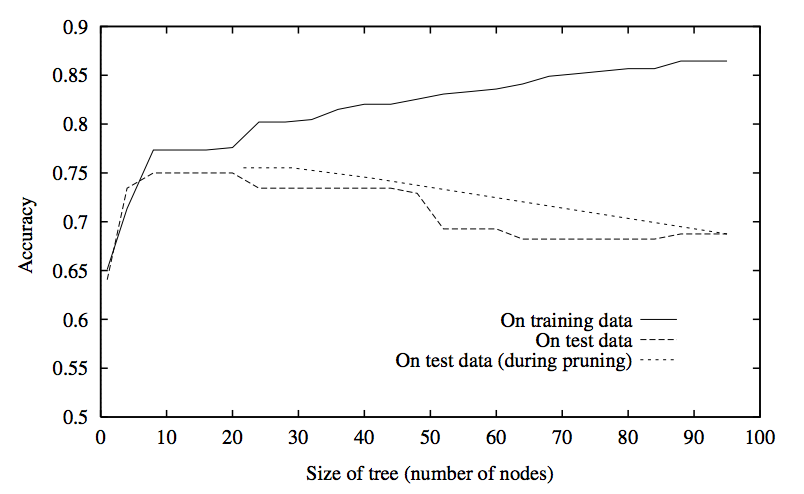
\includegraphics[width=.7\linewidth]{img/pruning}
\end{figure}


\chapter{Neural networks}
\section{Perceptron}
The perceptron is an algorithm for supervised learning of binary classifiers: functions that can decide whether an input (represented by a vector of numbers) belongs to one class or another.\\
\linebreak 
It is a type of linear classifier, i.e. a classification algorithm that makes its predictions based on a linear predictor function combining a set of weights with the feature vector. The algorithm allows for online learning, in that it processes elements in the training set one at a time. It is, in a way, akin to a linear discriminant.\\
\linebreak
Historically, it is also the first neural net inspired by human brain (which was then appearing as the best computer).

\paragraph{Associated learning} In a perceptron, the learning is supervised. It is based on a couple of input patterns and desired outputs. If the activation of output neuron corresponds to the desired output, nothing happens.
Otherwise, as inspired by neurophysiological data, if the neuron is activated: decrease the value of the connection and if it is unactivated: increase the value of the connection. This process is iterated until the output neurons reach the desired value. 
\begin{figure}[h]
    \centering
    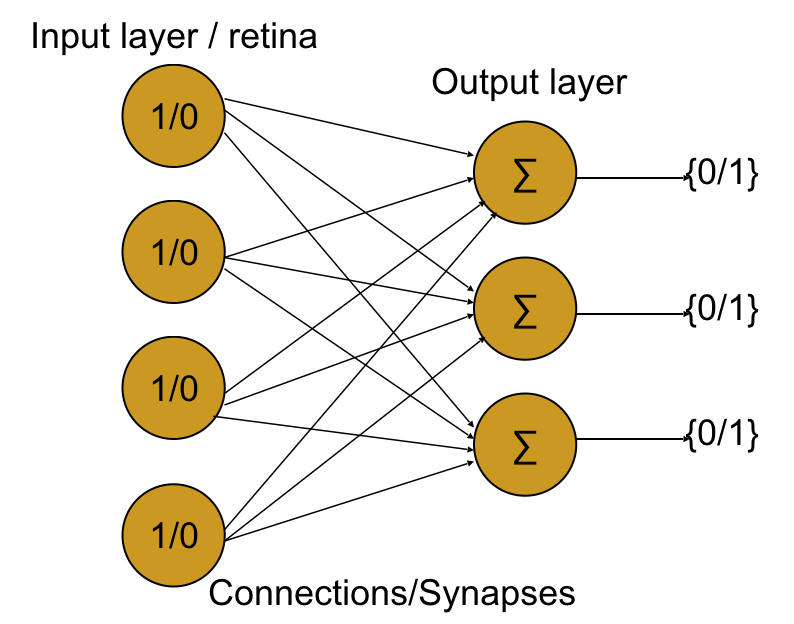
\includegraphics[width=.45\linewidth]{img/perceptron}
    \caption{Constitution of a perceptron}
\end{figure}
An approach to decreasing or increasing the value of  connections is the \textit{learning rule of Widrow-Hoff}. It considers the weight of a connection $w_{i, j}$, linking the output of neuron $i$ to the input of neuron $j$:
\begin{equation*}
    w_{i, j}^{t+1} = w_{i, j}^t + \eta (t_j - o_j) x_i = w_{i, j}^t + \Delta w_{i, j}
\end{equation*}
where $\eta$ is the learning rate, $t_j$ the target output of neuron $j$.
\begin{figure}[h]
    \centering
    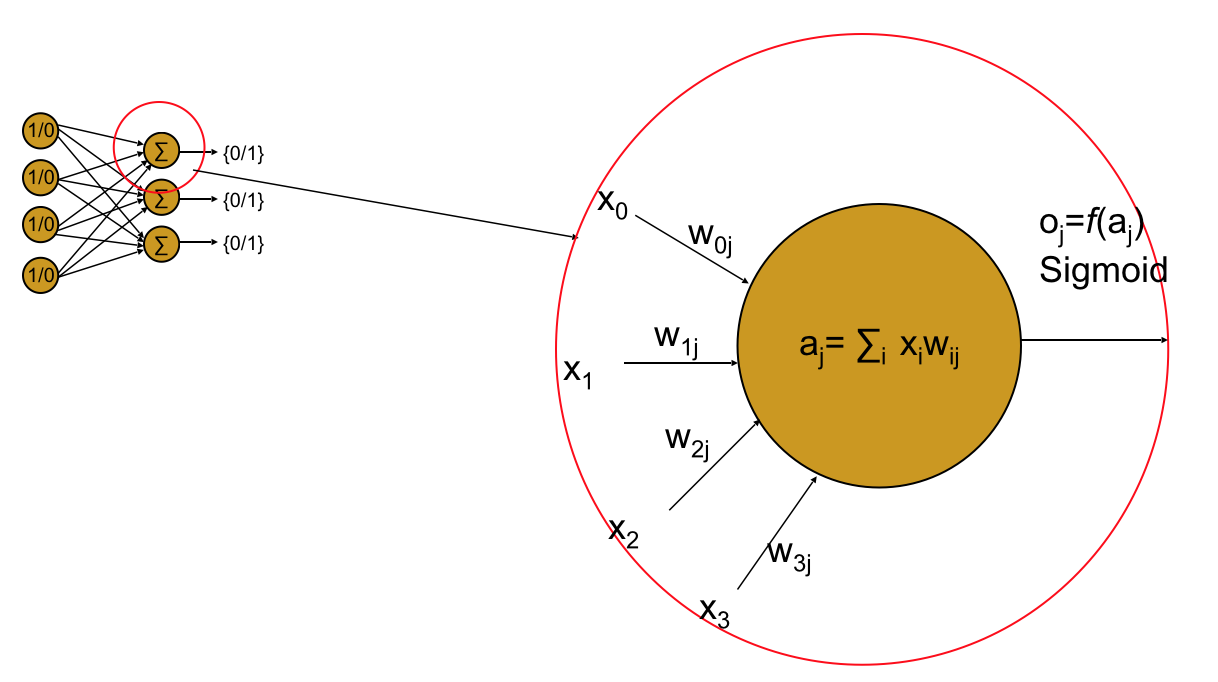
\includegraphics[width=.7\linewidth]{img/perceptron2}
    \caption{The neuron model. $x_i$ is the activation of the input neuron $i$, $a_j$ is the activation of the output neuron $j$, $w_{i, j}$ is the weight of the connection between neurons $i$ and $j$, and $o_j$ is the final output of the neuron, with respect to $a_j$ and the decision rule $f$. }
\end{figure}
At first, the decision rule function $f$ was chosen to be a step function with a certain threshold $b$, according to the data. That is:
\begin{equation*}
    f : x \mapsto y  = \begin{cases}1 & \text{if }w \cdot x + b > 0\\0 & \text{otherwise}\end{cases}
\end{equation*}
where $w \cdot x$ is the dot product $\sum_{i=0}^m w_i x_i$, and $m$ the number of inputs to the current neuron.
\paragraph{Gradient descent} It is a first-order optimization algorithm, used with perceptrons. To find a local minimum of a function, one will take steps proportional to the negative of the gradient (or of the approximate gradient) of the function at the current point. In most cases, a sigmoid is used, rather than a Heaviside (or step) function for the statistical interpretation:
\begin{equation*}
    f : x \mapsto y = \frac{1}{1 + e^{- x}}    
\end{equation*}
This function is interesting because its derivative is very easy to compute and therefore a good pick for the gradient descent technique:
\begin{equation*}
    f'=f(1-f)
\end{equation*}

\paragraph{Limitations of the perceptron} In some cases, the perceptron will not learn easily (if at all), as it cannot separate not linearly separable data. For example, the XOR gate, impossible to reproduce on a neural network, has killed all research on the subject for 20 years. Therefore, we had to wait for the magical hidden layer and for backpropagation for the perceptron to regain interest.

\section{Associative memories}
We will consider two types of associative memories:
\begin{itemize}
    \item Hetero-associative
    \item Auto-associative
\end{itemize}
We will treat here only auto-associative memories, which are also known as auto-association memories or an autoassociation networks. It is a generic term that refers to all memories that enable one to retrieve a piece of data from only a tiny sample of itself.\\
\linebreak
Traditional memory stores data at a unique address and can recall the data upon presentation of the complete unique address.\\
\linebreak 
Autoassociative memories are capable of retrieving a piece of data upon presentation of only partial information from that piece of data. Heteroassociative memories, on the other hand, can recall an associated piece of datum from one category upon presentation of data from another category.\\
\linebreak 
Hopfield networks have been shown to act as autoassociative memory since they are capable of remembering data by observing a portion of that data.\\
\linebreak
As a matter of example, the fragments presented below should be all that's necessary to retrieve the appropriate memory:\\
- "To be or not to be, that is \_\_\_\_\_" \\
- "I came, I saw, \_\_\_\_\_"\\
Readers will be able to complete the phrases above, given only a portion. The conclusion to be drawn is that autoassociation networks can recall the whole by using some of its parts.
\begin{figure}[h]
    \centering
    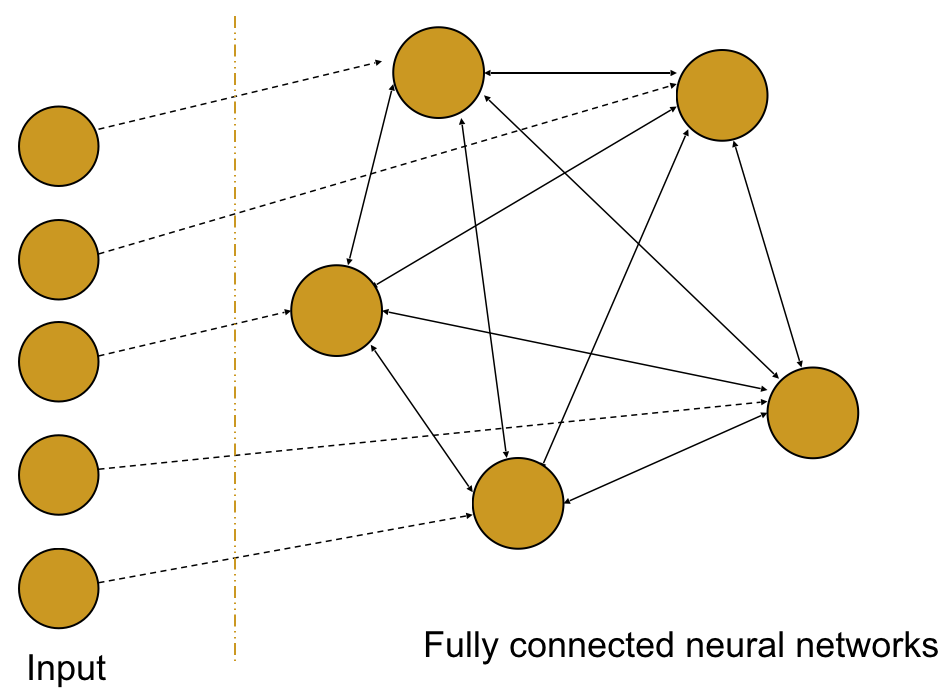
\includegraphics[width=0.5\linewidth]{img/associativememory}
    \caption{Constitution of an associative memory}
\end{figure}
\paragraph{Hopfield networks} They are a form of recurrent artificial neural network that serve as content-addressable memory systems with binary threshold nodes. They are guaranteed to converge to a local minimum, but convergence to a false pattern (wrong local minimum) rather than the stored pattern (expected local minimum) can occur. Hopfield networks also provide a model for understanding human memory.\\
\linebreak
The newtork becomes a dynamical machine, it has been shown to converge into a fixed point, which is of minimal Lyapunov energy. These fixed point are used for storing patterns.
\begin{figure}[h]
    \centering
    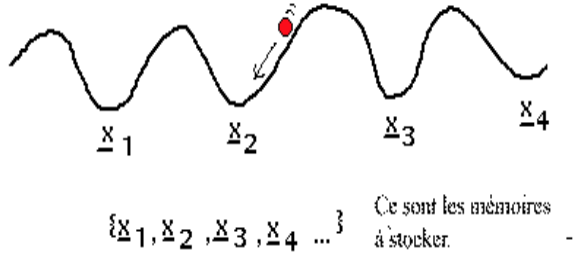
\includegraphics[width=0.35\linewidth]{img/mempatterns}
\end{figure}
We may then use a sort of gradient descent with:
\begin{equation*}
    \Delta W_{i, j} = \sum_{\text{patterns}} X^P_i X^P_j
\end{equation*}

\section{Multilayer perceptron}
To increase accuracy and extend the original perceptron abilities, we add one or more layers of neurons between the input and the output layers.
\begin{figure}[h]
    \centering
    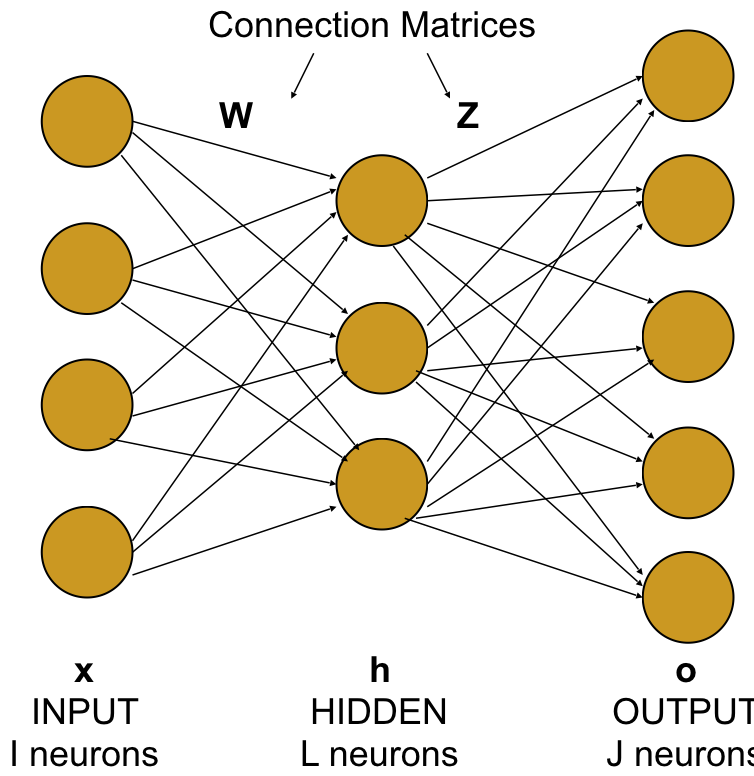
\includegraphics[width=0.35\linewidth]{img/multilayerperc}
\end{figure}
\begin{figure}[h]
    \centering
    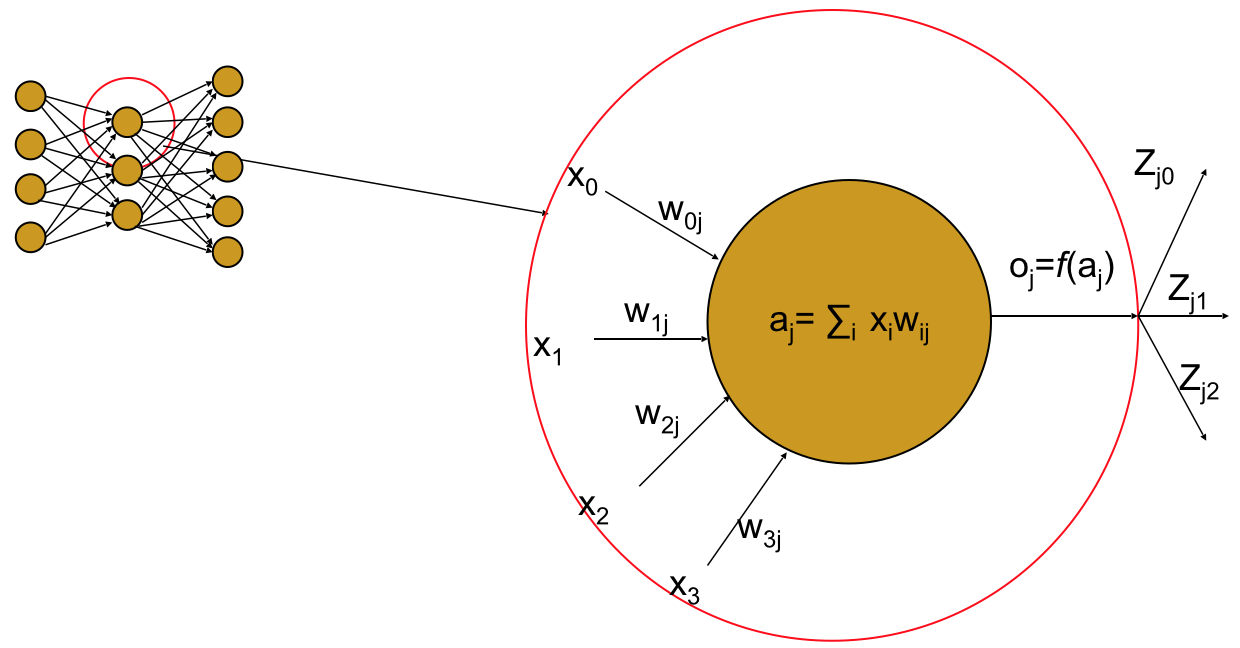
\includegraphics[width=0.7\linewidth]{img/multilayerperc2}
\end{figure}
Together with the multilayer perceptron come the backtracking technique and, more specifically, the backpropagation algorithm. It is a supervised learning method for multilayer networks, its name refers to the backward propagation of error during the training of the network. The algorithm is roughly described by the following steps:
\begin{algorithm}[caption={Neural network backtracking (main loop).}, label={alg11}]
inject an input $x$
compute the intermediate $h$: $ h = f(W \cdot x)$
compute the output $o$: $o = f(Z \cdot h)$
compute the error output $\delta_{out}$: $\delta_{out} = f'(Z \cdot h) * (t - o)$
adjust $z$ with respect to the error: $Z^{t+1} = Z^t + \eta * \delta_{out} * h = Z^t + \Delta^t Z$  
compute the error on the hidden layer: $\delta_{hidden} = f’(W \cdot x) * (Z \delta_{out})$
adjust $W$ with respect to this error: $W^{t+1} = W^t + \eta * \delta_{hidden} * h = W^t + \Delta^t W$
\end{algorithm}
\iffalse
\begin{enumerate}
    \item Inject an input $x$
    \item Compute the intermediate $h$:
    \begin{equation*}
        h = f(W \cdot x)
    \end{equation*}
    \item Compute the output $o$
    \begin{equation*}
        o = f(Z \cdot h)
    \end{equation*}
    \item Compute the error output $\delta_{out}$
    \begin{equation*}
        \delta_{out} = f'(Z \cdot h) * (t - o) 
    \end{equation*}
    \item Adjust $z$ with respect to the error
    \begin{equation*}
        Z^{t+1} = Z^t + \eta * \delta_{out} * h = Z^t + \Delta^t Z  
    \end{equation*}
    \item Compute the error on the hidden layer 
    \begin{equation*}
        \delta_{hidden} = f’(W \cdot x) * (Z \delta_{out})
    \end{equation*}
    \item Adjust $W$ with respect to this error
    \begin{equation*}
        W^{t+1} = W^t + \eta * \delta_{hidden} * h = W^t + \Delta^t W  
    \end{equation*}
    \item Repeat
\end{enumerate}
\fi
We can see it as a direct consequence of the chaining derivative of the gradient descent, where once again the sigmoid will come in handy. Also, we can show that in many cases, a neural network with more layers will produce more accurate results.

\chapter{Clustering}
Clustering is the process of grouping a set of instances (data points or
examples or vectors) into clusters (subsets or groups) so that instances
within a cluster have high similarity in comparison to one another, but
are very dissimilar to instances in other clusters.
Clustering may be found under different names in different contexts, such as:
\begin{itemize}
    \item Unsupervised learning
    \item Data segmentation
    \item Automatic classification
    \item Learning by observation
\end{itemize}
Similarities and dissimilarities of instances are based on the predefined features of the data. The most similar instances are grouped into a single
cluster.
\paragraph{Clustering instances} Let $X$ be the unlabelled data set, that is,
\begin{equation*}
    X = {x_1, x_2, ..., x_N}    
\end{equation*}
We may partition $X$ into $k$ clusters $C_1, ..., C_k$ so that the following conditions are met:
\begin{eqnarray*}
    C_i &\neq& \emptyset, ~\forall i \in [1, k] \\
    \cup_{i=1}^k C_i &=& X\\
    C_i \cap C_j &=& \emptyset, ~\forall i,j \in [1,k] \wedge i \neq j
\end{eqnarray*}

\paragraph{Requirements for clustering} The goal of clustering is to group a set of unlabelled data. There are many typical requirements of clustering in machine learning and data
mining, such as: 
\begin{itemize}
    \item Dealing with large data sets containing different types of attributes.
    \item Find the clusters with arbitrary shape.
    \item Ability to deal with noisy data in data streaming environment.
    \item Handling with high-dimensional data sets.
    \item Constraint-based clustering
\end{itemize}

\paragraph{Types of clustering methods}
The basic clustering methods are organised into the four categories:
\begin{enumerate}
    \item Partitioning methods
    \begin{itemize}
        \item The partitioning method constructs $k$ clusters of the given set of $N$
instances, where $k \leq N$. It finds mutually exclusive clusters of spherical shape using the traditional distance measures (Euclidean
distances).
        \item To find the cluster center, it may use mean or medoid (etc.) and apply iterative relocation technique to improve the clustering by moving instances from one cluster to another such as k-means
clustering.
        \item The partitioning algorithms are ineffective for clustering high-dimensional big data.
    \end{itemize}
    \item Hierarchical methods
    \begin{itemize}
        \item The hierarchical methods create a hierarchical decomposition of $N$ instances. It can be divided into two categories: the top-down (or divisive) approach, and the bottom-up (or agglomerative) approach.
        \item  The top-down approach starts with a single cluster having all the $N$ instances and then split into smaller clusters in each successive iteration, until eventually each instance is in one cluster, or a termination condition holds.
        \item The bottom-up approach starts with each instance forming a separate cluster and then successively merges the clusters close to one another, until all the clusters are merged into a single cluster, or a termination condition holds.
    \end{itemize}
    \item Density-based methods
    \begin{itemize}
        \item The density-based methods cluster instances based on the distance between instances, which can find arbitrarily shaped clusters. It can cluster instances as dense regions in the data space, separated by sparse regions.
    \end{itemize}
    \item Grid-based methods
    \begin{itemize}
        \item The grid-based methods use a multi-resolution grid data structure. It’s fast processing time that typically independent of the number of instances, yet dependent on the grid size        
    \end{itemize}
\end{enumerate}

\paragraph{Similarity measure} A similarity measure (SM), $sim(x_i, x_l)$, can be defined between any two instances $x_i, x_l \in X$, so that with an integer value $k$, the clustering problem is to define a mapping $f : X \mapsto [1, k]$, where each instance, $x_i$ is assigned
to one cluster $C_i$, with $1 \leq i \leq k$.\\
Given a cluster $C_i$:
\begin{equation*}
    sim(x_{il}, x_{im}) > sim(x_{il}, x_j), ~\forall x_{il}, x_{im} \in C_i \wedge x_j \notin C_i
\end{equation*}
A good clustering is that instances in the same cluster are “close” or related to each other, whereas instances of different clusters are “far
apart” or very different from one another, which together satisfy the following requirements:
\begin{itemize}
    \item Each cluster must contain at least one instance.
    \item Each instance must belong to exactly one cluster.
\end{itemize}

\paragraph{Distance measure} A distance measure (DM), $dis(x_i, x_l)$ where $x_i, x_l \in X$, is also often used in clustering. Let’s consider the
well-known Euclidean distance or Euclidean metric (i.e. straight-line) between two instances in Euclidean space:
\begin{equation*}
    dis(x_i, x_l) = \sqrt{\sum_{i = 1}^m(x_i - x_l)^2}
\end{equation*}
where $x_i = (x_{i1}, x_{i2}, ..., x_{im})$ and $x_l = (x_{l1}, x_{l2}, ..., x_{lm})$ are two
instances in Euclidean $m$-space.

\section{K-Means clustering}
It defines the centroid of a cluster, $C_i$ as the mean value of the instances $\{ x_{i1}, x_{i2}, ..., x_{iN} \} \in C_i$. It proceeds as follows:
\begin{enumerate}
    \item First, it randomly selects $k$ instances, $\{x_{k1}, x_{k2}, ..., x_{kN} \} \in X$ each of which initially represents a
cluster mean or center. 
    \item Each of the remaining instances, $x_i \in X$ is assigned to the cluster to which it is most similar, based on the Euclidean distance between the instance and the cluster mean. 
    \item It then iteratively improves the within-cluster variation. For each cluster, $C_i$, it computes the new mean using the instances assigned to the cluster in the previous iteration. All the instances, $x_i \in X$ are then reassigned into clusters using the updated means as the new cluster centers. \item The iterations continue until the assignment is stable, that is the clusters formed in the current round are the same as those formed in the previous round.
\end{enumerate}

\paragraph{Cluster mean} A high degree of similarity among instances in clusters is obtained, while a high degree of dissimilarity among instances in different clusters is achieved simultaneously. The cluster mean of $C_i = \{x_{i1}, x_{i2}, ..., x_{iN} \}$ is
defined by:
\begin{equation*}
    Mean = C_i = \frac{\sum^N_{j=1} x_{ij}}{N}
\end{equation*}

\begin{algorithm}[caption={k-Means clustering},label={alg12}]
$X \leftarrow {x_1, x_2, ... , xN }$, set of unlabelled instances.
$C \leftarrow {c_1, c_2, ... c_k}$, set of empty clusters
do until no change
    arbitrarily choose $k$ instances $x_i \in X$ as the initial $k$ clusters center
    (re)assign each $x_i$ to the $c_k$ with the most similar mean.
    update the $k$ means, that is, calculate the mean value of the instances for each cluster
\end{algorithm}

\paragraph{Drawbacks of k-means clustering} The k-Means clustering is not guaranteed to converge to the global optimum and often terminates at a local optimum (as the initial cluster means are assigned randomly). It may not be used in some application such as when data with nominal features are involved. The k-Means method is not suitable for discovering clusters with non-convex shapes or clusters of very different size. The time complexity of the k-Means algorithm is $O(nkt)$, where $n$ is the total number of instances, $k$ is the number of clusters, and $t$ is the number of iterations. Normally, $k \ll n$ and $t \ll n$.
\section{Similarity-based clustering}
A similarity-based clustering method (SCM) is an effective and robust clustering approach based on the similarity of instances, which is robust
to initialise the cluster numbers and efficient to detect different volumes of clusters. SCM is a method for clustering a data set into most similar
instances in the same cluster and most dissimilar instances in different clusters. The instances in SCM can self-organise local optimal cluster
number and volumes without using cluster validity functions.

\paragraph{Similarity between instances}
Let’s consider $sim(x_i, x_l)$ as the similarity measure between instances $x_i$ and the $l$th cluster center $x_l$. The goal is to find $x_l$ to maximise the total similarity measure:
\begin{equation*}
    J_s (C) = \sum_{l=1}^k \sum_{i=1}^N f(sim(x_i, x_l))
\end{equation*}
where, $f(sim(x_i, x_l))$ is a reasonable similarity measure and $C = \{ C_1, ..., C_k \}$. In general, the similarity-based clustering method uses feature values to check the similarity between instances. However, any suitable distance measure can be used to check the similarity
between the instances.
\begin{algorithm}[caption={Similarity-based clustering.}, label={alg13}]
$X \leftarrow \{ x_1, x_2, ..., x_N \}$
$C \leftarrow \emptyset$
$t \leftarrow $ threshold value
$k \leftarrow 1$
$C_k \leftarrow {x_1}$
$C \leftarrow C \cup C_k$
for $i = 2$ to $N$ do
    for $l = 1$ to $k$ do
        find the $l$th cluster center $x_l \in C_l$ to maximize the similarity
measure, $\text{arg~max}_{x_l} sim(x_i, x_l)$
    if $sim(x_i, x_l) \geq t$ then
        $C_l \leftarrow C_l \cup x_i$
    else
        $k \leftarrow k+1$
        $C_k \leftarrow \{ x_i \}$
        $C \leftarrow C \cup C_k$
return C
\end{algorithm}
\section{Nearest neighbor clustering}
Instances are iteratively merged into the existing clusters that are closest. In NN clustering a threshold, $t$, is used to determine if instances will be added to existing clusters or if a new cluster is created. The complexity of the NN clustering algorithm is depends on the number of instances in the dataset. For each loop, each instance must be compared to each instance already in a cluster. Thus, the time complexity of NN clustering algorithm is $O(n^2)$. We do need to calculate the distance between instances often, we assume that the space requirement is also $O(n^2)$.
\begin{algorithm}[caption={Nearest-neighbor clustering.}, label={alg14}]
$D \leftarrow \{ x_1, x_2, ..., x_n \}$
$A \leftarrow$ adjacency matrix showing distance between instances
$t \leftarrow$ threshold value
$C_1 \leftarrow \{x_1\}$
$C \leftarrow \{C_1\}$
$k \leftarrow 1$
for $i = 2$ to $n$
    $x_m = \text{arg min}~dis(x_i, x_m) \forall x_m \in C_j, ~\forall C_j \in C$
    if $dis(x_i, x_m) \leq t$
        $C_m \leftarrow C_m \cup x_i$
    else
        $k \leftarrow k + 1$
        $C_k \leftarrow \{ x_i \}$
        $C \leftarrow C \cup C_k$
return $C$
\end{algorithm}

\paragraph{Euclidean vs Manhattan distance} The distance between the two points in the plane with coordinate $(x,y)$ and $(a,b)$ is given by:
\begin{eqnarray*}
    EuclideanDistance((x,y), (a,b)) &=& \sqrt{(x-a)^2 + (y-b)^2} \\
    ManhattanDistance((x,y),(a,b)) &=& |x-a| + |y-b|
\end{eqnarray*}


\section{Ensemble clustering}
Ensemble clustering is a process of integrating multiple clustering algorithms to form a single strong clustering approach that usually provides better clustering results. It generates a set of clusters from a given unlabelled data set and then combines the clusters into final clusters to improve the quality of individual clustering.
\begin{itemize}
    \item No single cluster analysis method is optimal.
    \item Different clustering methods may produce different clusters, because they impose different structure on the data set.
    \item Ensemble clustering performs more effectively in high dimensional complex data.
    \item It’s a good alternative when facing cluster analysis problems.
\end{itemize}
Generally three strategies are applied in ensemble clustering: 
\begin{enumerate}
    \item Using different clustering algorithms on the same data set to create heterogeneous clusters.
    \item Using different samples/ subsets of the data with different clustering algorithms to cluster them to produce component clusters.
    \item Running the same clustering algorithm many times on same data set with different parameters or initialisations to create homogeneous clusters.
\end{enumerate}
The main goal of the ensemble clustering is to integrate component clustering into one final clustering with a higher accuracy.

\section{Subspace clustering}
The subspace clustering finds subspace clusters in high-dimensional data. It can be classified into three groups:
\begin{enumerate}
    \item Subspace search methods.
    \item Correlation-based clustering methods
    \item Biclustering methods.
\end{enumerate}
A subspace search method searches various subspaces for clusters (set of instances that are similar to each other in a subspace) in the full space. It uses two kinds of strategies: 
\begin{enumerate}
    \item Bottom-up approach - start from low-dimensional subspace and search higher-dimensional subspaces.
    \item Top-down approach - start with full space and search smaller subspaces recursively.
\end{enumerate}
A correlation-based approach uses space transformation methods to derive a set of new, uncorrelated dimensions, and then mine clusters in the new space or its subspaces. It uses PCA-based approach (principal components analysis), the Hough transform, and fractal dimensions. Biclustering methods cluster both instances and features simultaneously, where cluster analysis involves searching data matrices for sub-matrices that show unique patterns as clusters.

\chapter{Evaluation of hypothesis}
\section{Two definitions of the error}
The \textbf{true error} of hypothesis $h$ with respect to target function $f$ and distribution $\mathcal{D}$ is the probability that $h$ will misclassify an instance drawn at random according to $\mathcal{D}$.
\begin{eqnarray}
error_{\mathcal{D}}(h) \equiv \text{Pr}  _{x \in \mathcal{D}}  [ f(x) \neq h(x) ]	
\end{eqnarray}
The \textbf{sample error} of hypothesis $h$ with respect to target function $f$ and data sample $S$ is the proportion of examples $h$ misclassifies.
\begin{eqnarray}
error_{S}(h) \equiv \frac{1}{n} \sum_{x \in S} \delta (f(x) \neq h(x))	
\end{eqnarray}

\section{Estimators}
\paragraph{Problems estimating error} There are two problems to keep in mind:
\begin{enumerate}
	\item Bias: if $S$ is a training set, $error_S(h)$ is optimistically biased:
	\begin{eqnarray}
		bias \equiv E [error_S(h)] - error_{\mathcal{D}}(h)
	\end{eqnarray}
	To get an unbiased estimate, $h$ and $S$ must be chosen independently.
	\item Variance: even with an unbiased training set $S$, $error_S(h)$ may still vary from $error_{\mathcal{D}}(h)$.
\end{enumerate}
For example, if $h$ misclassifies 12 of the 40 examples in $S$, $error_S(h) = 12/40 = .3$.
\section{Confidence intervals for observed hypothesis error}
Let's go through all this section with a quick example. If the training set $S$ contains $n$ examples, drawn independently of $h$ and each other and $h \geq 30$, then $error_\mathcal{D}(h)$ lies with $N$\% probability in the interval:
\begin{eqnarray}
	error_S(h) \pm z_N \sqrt{\frac{error_S(h)(1 - error_S(h))}{n}}
\end{eqnarray}  
where the pairs ($N, z_N$) are the usual $(50, 0.67), (68, 1.00)$, $(80, 1.28)$, $(90, 1.64)$, (95, 1.64), $(98, 2.33)$, $(99, 2.58)$.
\section{Binomial distribution, normal distribution and central limit theorem}
Same old same old.. In short:
\begin{enumerate}
	\item Pick parameter $p$ to estimate $error_{\mathcal{D}} (h)$
	\item Choose an estimator $error_S(h)$
	\item Determine probability distribution that governs estimator $error_S(h)$ governed by Binomial distribution, approximated by Normal when $n \geq 30$.
	\item Find interval $(L, U)$ such that $N$\% of probability mass falls in the interval: use table of $z_N$ values.

\end{enumerate}

\section{Paired $t$ tests}
\begin{enumerate}
	\item Partition data into $k$ disjoint test sets $T_1, T_2, ..., T_k$ of equal size, where this size is at least 30.
	\item For $i$ from 1 to $k$, do 
	\begin{eqnarray}
		\delta_i \leftarrow error_{T_i} (h_A) - error_{T_i} (h_B)
	\end{eqnarray}
	\item Return the value $\bar{\delta}$, where
	\begin{eqnarray}
		\bar{\delta} \equiv \frac{1}{k} \sum^{k}_{i = 1} \delta_i 
	\end{eqnarray}
\end{enumerate}
The confidence interval ($N$\%) estimate for $d$ becomes
\begin{eqnarray}
	\bar{\delta} &pm& t_{N, k-1} s_{\bar{\delta}} \\
	s_{\bar{\delta}} &\equiv& \sqrt{\frac{1}{k(k-1)} \sum^{k}_{i = 1} (\delta_i - \bar{\delta})^2}
\end{eqnarray}
$\bar{\delta}$ is said to be approximately normally distributed.
\section{Comparing learning methods}
The idea is only to compute the errors of various learning algorithms and estimate their difference.
\chapter{Data, text and graph mining}
Data mining is an interdisciplinary subfield of computer science. It is the computational process of discovering patterns in large data sets involving methods at the intersection of artificial intelligence, machine learning, statistics, and database systems. The overall goal of the data mining process is to extract information from a data set and transform it into an understandable structure for further use.
\section{Data warehouses}
\paragraph{Preparing the data} It is a key step in the data mining process. Data has to be clean and homogeneous. Different variables must be expressed on the same scale, etc. You need to have regularities in the data.

\paragraph{The main techniques of data mining}
\begin{itemize}
    \item Clustering (unsupervised, only group the data)
    \item Outlier detection (check if some data is \textit{unusual}, e.g. detect fraud - many ways to be dishonest and few ways to be honest)
    \item Association analysis (discovering interesting relationships hidden between various items of large data sets)
    \item Forecasting
    \item Classification
\end{itemize}
Note the difference between classification and clustering: in classification you have a set of predefined classes and want to know which class a new object belongs to. Clustering tries to group a set of objects and find whether there is some relationship between the objects.

\section{Understanding and predicting data}
Basically, we define a vector space, formatting our graph/text/image/whatever type of data it is as an $n-$dimensional, normalized (and why not some other interesting properties) vector.
\section{Data mining techniques}

\chapter{Metaheuristics: genetic algorithms}
Genetic Algorithms and Ant Colony Optimisation

\chapter{Reinforcement Learning}
(Chapter 13 Tom Mitchell)
(slides used during the lecture)
\chapter{Recommender Systems}
\end{document}